\chapter{Experiments and Results}\label{results}

In chapter we describe the experiments performed with the Word2Vec-ESN model and the variant proposed in the previous chapter. The results obtained by the Word2Vec-ESN model, using word embeddings, are compared with $\theta RARes $ model which uses sentence in grammatical form by replacing semantic word with 'SW' token and localist representation of words.

\section{Input and Ouput Coding}

\paragraph{Word2Vec-ESN model:} A raw sentence is presented to the model, where each word in the sentence is processed across time by both word2vec model and ESN. The word2vec model outputs the $E_{v}=50$ dimension word embedding which is then used as input for ESN. Thus input layer have 50 neurons. For the experiment with corpus-462 we used a reservoir of $1000$ leaky integrator neurons with \textit{tanh} activation fuction. For the output coding the topologically modified but equivalent representation is used \cite{xavier:2013:RT}. Thus, the readout layer contains 24 $(4 \times 3 \times 2)$ neurons as the corpus contains sentences having maximum of 4 nouns each having 3 possible roles (Agent, Object and Recipient) with respect to a maximum of 2 verbs. Output neuron have an activation 1 if the role is present in the sentence, -1 otherwise. Whereas when using corpus-90582 for training the number of neurons in reservoir were raised to 5000 and also the  readout neurons are increased to 30 $(5 \times 3 \times 2)$ as there were maximum of 5 nouns in the sentences of this corpus.

\paragraph{Word2Vec-ESN model variant:} In the Word2Vec-ESN model variant a raw sentence is presented to the model, where each word (argument) along with the verb (Predicate) with respect to which the word is currently processed, is input to the model across time(see section \ref{sec:model_variant}). A sentence is processed as many time as there are verbs in the sentence. The word2vec model firstly takes this argument-predicate pair as an input and outputs a vector of $E_{v}=2 \times 50$ dimension, which is then used as an input to ESN. Thus input layer thus have 100 neurons where first 50 neurons encodes the vector representation of the word and remaining 50 neurons codes for the verb with respect to which word is processed. The reservoir of size 1000, 3000 is used for corpus-462 and corpus-90582 respectively. Unlike the model variant-1, the size of readout neurons always remains the same and contains 5 neurons each coding for a role: Predicate (P), Agent(A), Object(O), Recipient(R) and No Role(XX). Readout neuron of ESN have an activation 1 if the input word-verb (argument-predicate) pair have the corresponding role, -1 otherwise.

\section{Experiments}

\subsection{Experiment-1: Learning thematic roles}

In order to determine the model capability for predicting thematic roles of the sentences using word2vec embeddings for words, we first did the experiment using 26 sentences(sentence 15 to 40, in corpus-45) from corpus-45. The chosen sentences have distinct surface form (e.g. active, passive, dative-passive) and grammatical structure. This also include the sentences with single verb or double verb relative surface form [ref?]. Both the model variants(see section-?) learned the sentences without any error when trained and tested on all the sentences. To test the performance and generalization capabilities of model on untrained sentences, we performed a leave-one-out cross validation, where a model is trained on 25 sentences out of 26 and tested on remaining 1 sentence.

\paragraph{Model Variant-1:} The model variant-1 with a reservoir of size 1000 units the model yielded [?] meaning error and [?] sentence error in sentence continuous learning mode and [?] meaning error and [?] sentence error in Sentence final learning mode. The results were averaged over 10 reservoir instances. For Continuous learning model the spectral radius(SR), input scaling (IS) and leak rate($\alpha$) were identified as $SR=[?], IS=[?], \alpha=[?]$.` Whereas for Sentence final learning mode the $SR=?, IS=?, \alpha=?$. The ESN parameters for which the optimized results are identified are found by exploration of parameter space. As one may note that difference in training and test error for both meaning and sentence error is large. This indicates the model is overfitting on the dataset. However, it is not surprisring because the dataset contains limited examples, which constrained model to generalize well. As this experiments remains a toy demonstration we will explore the generalization capabilty of the model in section \ref{exp-2} .

\paragraph{Model Variant-2:} The model Variant-2, on the other hand, with a reservoir of size 600 neurons, produced the classification scores [write score here] during cross-validation. 

\subsection{Experiment-2: Generalization Capabilities} \label{exp-2}

In the previous experiment we demonstrated the performance of the model with the limited set of sentences where the results suggested that the model is probably overfitting and not generalizing on the unseen sentences. So in order to test the generalization capability of the model, we examined the model's behaviour with an extended corpus of 462 sentences (see corpus-462 in \ref{datasets}) using 10-fold cross validation. Corpus-462 with 462 sentences was randomly split into 10 equally sized subsets(i.e. each subset with $\approx$ 46 sentences). The model was trained on sentences from 9 subsets and then tested on remaining one subset. This process was repeated 10 times such that the model is trained and tested on all the subsets atleast once. 

\paragraph{Word2Vec-ESN:} We initially trained and tested the model with reservoir of 1000 neurons on all the 462 sentences. The model learned the full corpus-462 with $0.54\%$ meaning error and $1.51\%$ sentence error in SCL mode and $0.14\%$ meaning error and $0.43\%$ sentence error in SFL mode. Using the 10-fold cross validation, the model generalized to $7.82\% (\pm 1.59\%) $ meaning error and $20.65\% (\pm 2.79\%)$ sentence error in SCL mode with spectral radius (SR), input scaling (IS) and leak rate(LR) of $2.4$, $2.5$ and $0.07$ respectively. Whereas in the SFL mode with $SR = 2.2$, $IS = 2.3$ and $LR = 0.13$, the optimal meaning and sentence error were observed as $8.68\% (\pm 1.26\%)$ and $23.69\% (\pm 1.17\%)$ respectively. The optimal parameters for both the learning models (SCL and SFL) were identified using grid search over the parameter space.

We compared the performance of Word2Vec-ESN model with $\theta RARes$ model which takes the sentences in grammatical form and words are represented in localist fashion. As illustrated in table \ref{tab:corpus-462_errors}, during testing, we observed an improvement of $11.48 \%$ sentence error in SCL mode with Word2Vec-ESN model whereas meaning error remained almost equivalent in both the models. In SFL mode, using Word2Vec-ESN model, both meaning and sentence errors dropped nearly by $1 \%$. One can also notice that with Word2Vec-ESN model, the performance gain in more in SCL mode as compared to SFL mode. The reason is that the word-embeddings in word2vec model are learned from the context words and thus word vector encapsulates the information about neighbouring words.  

%NOTE: 08/09/2016 results are copied after the simulation and are final, no need to change.
\begin{table}
\centering
\begin{threeparttable}
\caption{Mean and standard deviation of meaning and sentence error on train and test set of coprus-462 in different learning modes.}
\label{tab:corpus-462_errors}
\rowcolors{2}{white}{gray!25}
\begin{tabularx}{\textwidth}{@{}llYYYY@{}}
  \toprule
  &  & \multicolumn{2}{c}{Word2Vec-ESN} & \multicolumn{2}{c}{$\theta RARes$} \\
  \cmidrule(lr){3-4}   \cmidrule(lr){5-6}
  \hiderowcolors   
  
  						& 		& ME 	& SE 			& ME 	& SE 		\\
  \midrule
  \showrowcolors
  \textbf{SCL\ train} 	& mean 	& 0.541 & 1.515 	 	& 0.123 & 1.207 	\\
   			    		& std 	& 0.000 & 0.000 	 	& 0.029 & 0.297 	\\
   			    		
  \textbf{SCL\ test} 	& mean  & 7.826 & 20.652 	 	& 7.433 & 32.130 	\\
  			   			& std  	& 1.598 & 2.792 	  	& 0.534 & 1.353 	\\
  			   			
  \textbf{SFL\ train} 	& mean 	& 0.144 & 0.432 	 	& 0.000 & 0.000 	\\
  				 		& std 	& 0.000 & 0.000 	 	& 0.000 & 0.000 	\\
  				 		
  \textbf{SFL\ test}	& mean  & 8.686 & 23.695 	 	& 9.178 & 24.370 	 \\
  			  			& std 	& 1.265 & 1.170		  	& 0.574 & 1.192 	  \\
  \bottomrule
\end{tabularx}
\begin{tablenotes}
\small
\item 
Meaning (ME) and Sentence error (SE) in different learning modes with Word2Vec-ESN model using distributed word embeddings and $\theta RARes$ \cite{xavier:2013:RT} model which uses grammatical form and localist representation of words of sentences. The errors are given in percentage. SFL:Sentence Continuous learning; SFL: Sentence Final Learning; std: Standard Deviations. Simulations were done with reservoir of 1000 neurons.
\end{tablenotes}
\end{threeparttable}
\end{table}
	
\paragraph{Word2Vec-ESN Variant:} The word2vec-ESN model variant with a reservoir of size 1000 neurons when trained and tested on all 462 sentences of corpus-462, learned to label the word in the sentences with an Accuracy(Ac), Precision(Pr), Recall(Re) and F1-Score(F1) of $97.38\%$,  $97.48\%$, $92.28\%$, $94.64\%$ respectively. When the model variant was tested using 10-fold cross validation we got Ac = $97.18\% (\pm 0.11\%)$, Pr = $96.86\% (\pm 0.49\%)$, Re = $91.93\% (\pm 0.23\%)$ and F1 = $94.16\%(\pm 0.26\%)$ with $IS=1.15, SR=0.7, LR=0.1$. The marginal difference between the training and cross validation scores indicates that the model variant is generalizing well even on untrained data and is not overfitting. The precision, recall and f1-score for individual role is listed in table \ref{tab:classsification-scores-21}. 

\begin{table}
\centering
\begin{threeparttable}
\caption{Training and testing classification scores for individual roles when using Word2Vec-ESN model variant.}
\label{tab:classsification-scores-21}
\rowcolors{2}{gray!25}{white}
\begin{tabularx}{\textwidth}{@{}llYYYYYYY@{}}
\hiderowcolors
\toprule
  &  & \multicolumn{3}{c}{word2vec vectors} & \multicolumn{3}{c}{GF \& localist vectors}& \\  
\cmidrule(lr){3-5}   \cmidrule(lr){6-8}
   
Role 				& 		& Pr   & Re  & F1 		& Pr  &  Re & F1 		&  Support  \\
\showrowcolors
\midrule
               
\textbf{Agent}		&test 	& 0.92 & 0.79 & 0.85 	& 0.66 & 0.62 & 0.64	& 888 \\
					&train  & 0.94 & 0.80 & 0.86 	& 0.71 & 0.68 & 0.69	& 892 \\
\textbf{Object}		&test 	& 0.95 & 0.81 & 0.88 	& 0.61 & 0.65 & 0.63	& 791 \\
					&train  & 0.96 & 0.81 & 0.88 	& 0.67 & 0.69 & 0.68	& 794 \\
\textbf{Recipient}	&test 	& 1.00 & 1.00 & 1.00 	& 0.69 & 0.96 & 0.80	& 383 \\
					&train  & 1.00 & 1.00 & 1.00 	& 0.70 & 0.97 & 0.81	& 384 \\
\textbf{Predicate}	&test	& 1.00 & 1.00 & 1.00 	& 0.96 & 0.92 & 0.94	& 888 \\
					&train  & 1.00 & 1.00 & 1.00 	& 0.98 & 0.94 & 0.96	& 892 \\
\textbf{No Role}	&test 	& 0.97 & 1.00 & 0.99 	& 0.97 & 0.96 & 0.97	& 9785 \\
					&train  & 0.97 & 1.00 & 0.99 	& 0.98 & 0.97 & 0.97	& 9823 \\
\bottomrule
\end{tabularx}
\begin{tablenotes}
\small
\item Comparision of training and cross validation scores for each output roles predicted by the model. Support for each role: actual number of instance, is also shown in last column. Simulation were done using 1000 reservoir neurons and parameters: SR = 0.7, IS = 1.15, LR = 0.1.
\end{tablenotes}
\end{threeparttable}
\end{table}

We also performed the simulations using Word2Vec-ESN model variant with grammatical form of sentences with localist word representation. The model produced Pr = $80.60 \%$, Re = $84.90 \%$, F1 = $82.31 \%$ during training and Pr = $78.04 \%$, Re = $82.23 \%$, F1 = $79.68 \%$ during cross-validation. 

% analyse table and confusion matrix
[Confusion matrix to be analyzed]

\begin{figure}[hbtp]
\centering
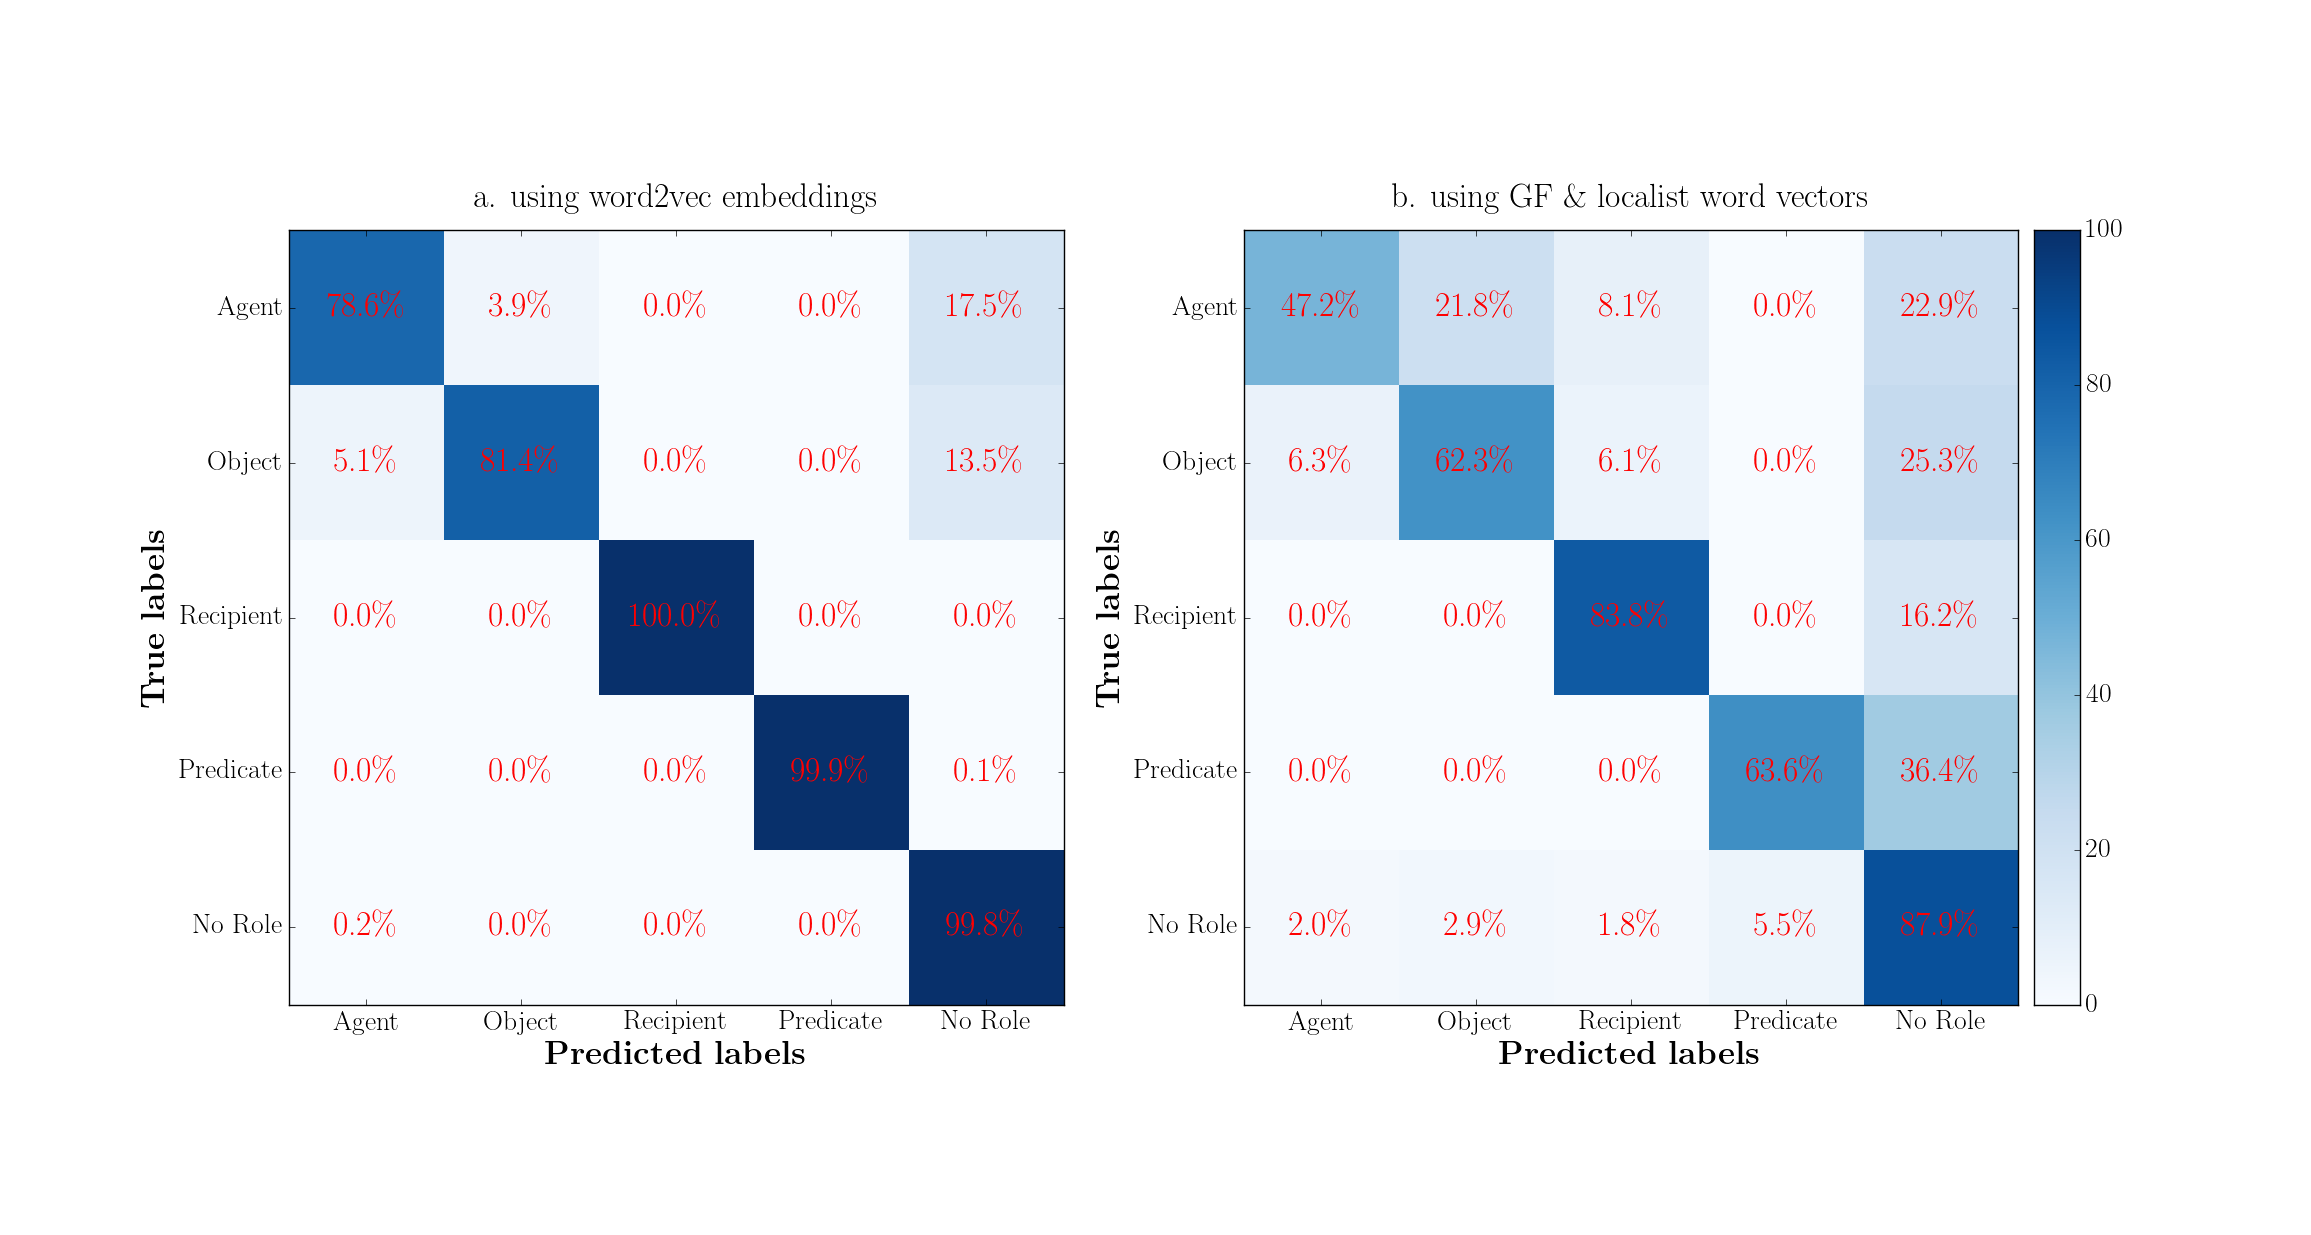
\includegraphics[width=1.0\linewidth]{confusion_matrix}
\caption[Normalized confusion matrix on corpus 462 with Word2Vec-ESN model variant] {\textbf{Normalized confusion matrix with Word2Vec-ESN model variant:} The confusion matrix with true roles (in rows) and predicted roles (in columns). The top-left to bottom-right diagonal shows the percentage of words whose roles are predicted correctly. Everything other than this diagonal represents the incorrect prediction of roles. Model identified almost all words labelled as Recipient , Predicate and No Role and made some errors in predicting role Agent and Object. The results were obtained with reservoir of 1000 neurons and 10 fold-cross validation.}
\label{fig:confusion_matrix}
\end{figure}


\subsection{Experiment-3: Effect of Corpus structure} 

Recall that the sentences in the corpus-462 was created based on context free grammer. Thus the sentences in the corpus contains inherent grammatical structure. The model is thus possibly utilizing the underlying grammatical structure to some extend for learning and generalizing. To test this hypothesis and to demonstrate that the model is not generalizing on any other inconsitent regularity in the corpus, we removed the inherent grammatical structure from the sentence in the corpus by randomizing the word orders within the sentences \cite{xavier:2013:RT}. Such a test will also help us to have insight on what the model is actually learning and whether the model is overfitting or not. The situation of overfitting typically occurs when the corpus size is significantally less than the number of trainable parameters \cite{xavier:2013:RT}. The Word2Vec-ESN model with reservoir of size 1000 neurons and 42 readout neurons have 42000 $(42 \times 1000)$ trainable parameters, whereas the model variant with reservoir size $1000$ and $5$ readout neuron the trainable parameters are 5000 $(5 \times 600)$. In both the case the number of trainable parameters are significantally greater than our corpus size (i.e. 462 sentence). This is thus a possible situation of overfitting.

We presented the corpus with the scrambled sentences(i.e. in absence of any grammatical structure) to both Word2Vec-ESN model and its variant and performed a 10 fold cross-validation. The cross validation errors obtained in the previous experiment on the corpus with inherent grammatical structure can then be compared with the cross validation error obtained while using scrambled corpus. If the model is not overfitting and learning from the grammatical structure then the model should generalize better for the corpus with unscrambled sentences (i.e. in presence of grammatical structure). However in case of overfitting the generalization effect should not vary much both in presence and absence of grammatical structure in the corpus.

As illustrated in Table.[no], we observed that [analysis to follow....]

\begin{table}
\centering
\begin{threeparttable}
\caption{Mean and standard deviation of meaning and sentence error on train and test set of coprus-462 in different learning modes.}
\label{tab:corpus-structure}
\rowcolors{2}{white}{gray!25}
\begin{tabular}{llcccc}
  \toprule
  &  & \multicolumn{2}{c}{Word2Vec-ESN} & \multicolumn{2}{c}{$\theta RARes$} \\
  \cmidrule(lr){3-4}   \cmidrule(lr){5-6}   
  
  						& 			& ME 		& SE 			& ME 	 & SE \\
  \midrule
  \textbf{SCL\ train} 	& mean 	 	& 7.312 	& 30.303 	 	& 4.813  & 20.433  \\
   			    		& std 	 	& 0.000 	& 0.000 	 	& 0.299  & 1.251  \\
   			    		
  \textbf{SCL\ test} 	& mean   	& 69.761	& 99.130 	 	& 74.154 & 99.891 \\
  			   			& std  	 	& 1.462  	& 1.064  	 	& 0.802  & 0.146\\
  			   			
  \textbf{SFL\ train} 	& mean 	 	& 9.148  	& 31.168 	 	& 0.000  & 0.000  \\
  				 		& std 	 	& 0.000  	& 0.000 	 	& 0.000  & 0.000  \\
  				 		
  \textbf{SFL\ test}	& mean   	& 67.548 	& 99.347 	 	& 73.391 & 99.913 \\
  			  			& std 		& 1.971  	& 0.996  	 	& 0.962  & 0.106  \\
  \bottomrule
\end{tabular}
\begin{tablenotes}
\small
\item 
Meaning (ME) and Sentence error (SE) in different learning modes with our approach of using word2vec embeddings and Xavier's \cite{xavier:2013:RT} approach of using grammatical construction and localist representation of words. The errors are given in percentage. For Sentence Final Learning mode (SFL): our approach (IS = 2.3, SR = 2.3, LR = 0.13 ) and Xavier's approach(IS = 1, SR =, LR =). For Sentence Continuous Learning mode (SCL): our approach (IS=2.5, SR=2.4, LR=0.07) and Xavier's approach(SR = 1,LR = ). Simulation were done with 10 reservoir instance of 1000 neurons.
\end{tablenotes}
\end{threeparttable}
\end{table}

\subsection{Experiment-4: Effect of Reservoir size}

One of the important hyperparmeter which effects the performance of the model is the size of reservoir (i.e. number of neurons in the reservoir). Also the addition of neurons in the reserovir is computationally inexpensive, because the read-out weights ($W^{out}$) scales linearly with the number of neurons in the reservoir[ref?]. So, in order to determine the effect of reservoir size on the peformance of the model variant-1, we plotted the cross validation errors (see fig. \ref{fig:reservoir_size_1}) against the number of neurons in the reservoir. 

It was observed that both meaning and sentence cross validatoin error reduces with increase in reservoir size but asymptotes when the reservoir size is above 1000 neurons for this corpus (i.e. corpus-462). This indicates that the model can not generalize further for this corpus with further increase in reservoir size. However the lowest errors were observed in reservoir with 2882 neurons with meaning and sentence error of $6.74 \% (\pm 1.5\%)$ and $17.39\% (\pm 4.23 \%)$ in SCL mode. In SFL model meaning error and sentence errors were observed as $8.70 \% (\pm 1.62\%)$ and $22.60\% (\pm 5.25 \%)$ respectively. It can be noticed that these lowest errors does not vary significantally when compared to errors obtained with reservoir of size 1000 neurons (see table \ref{tab:corpus-structure}).

\begin{figure}[hbtp]
\centering
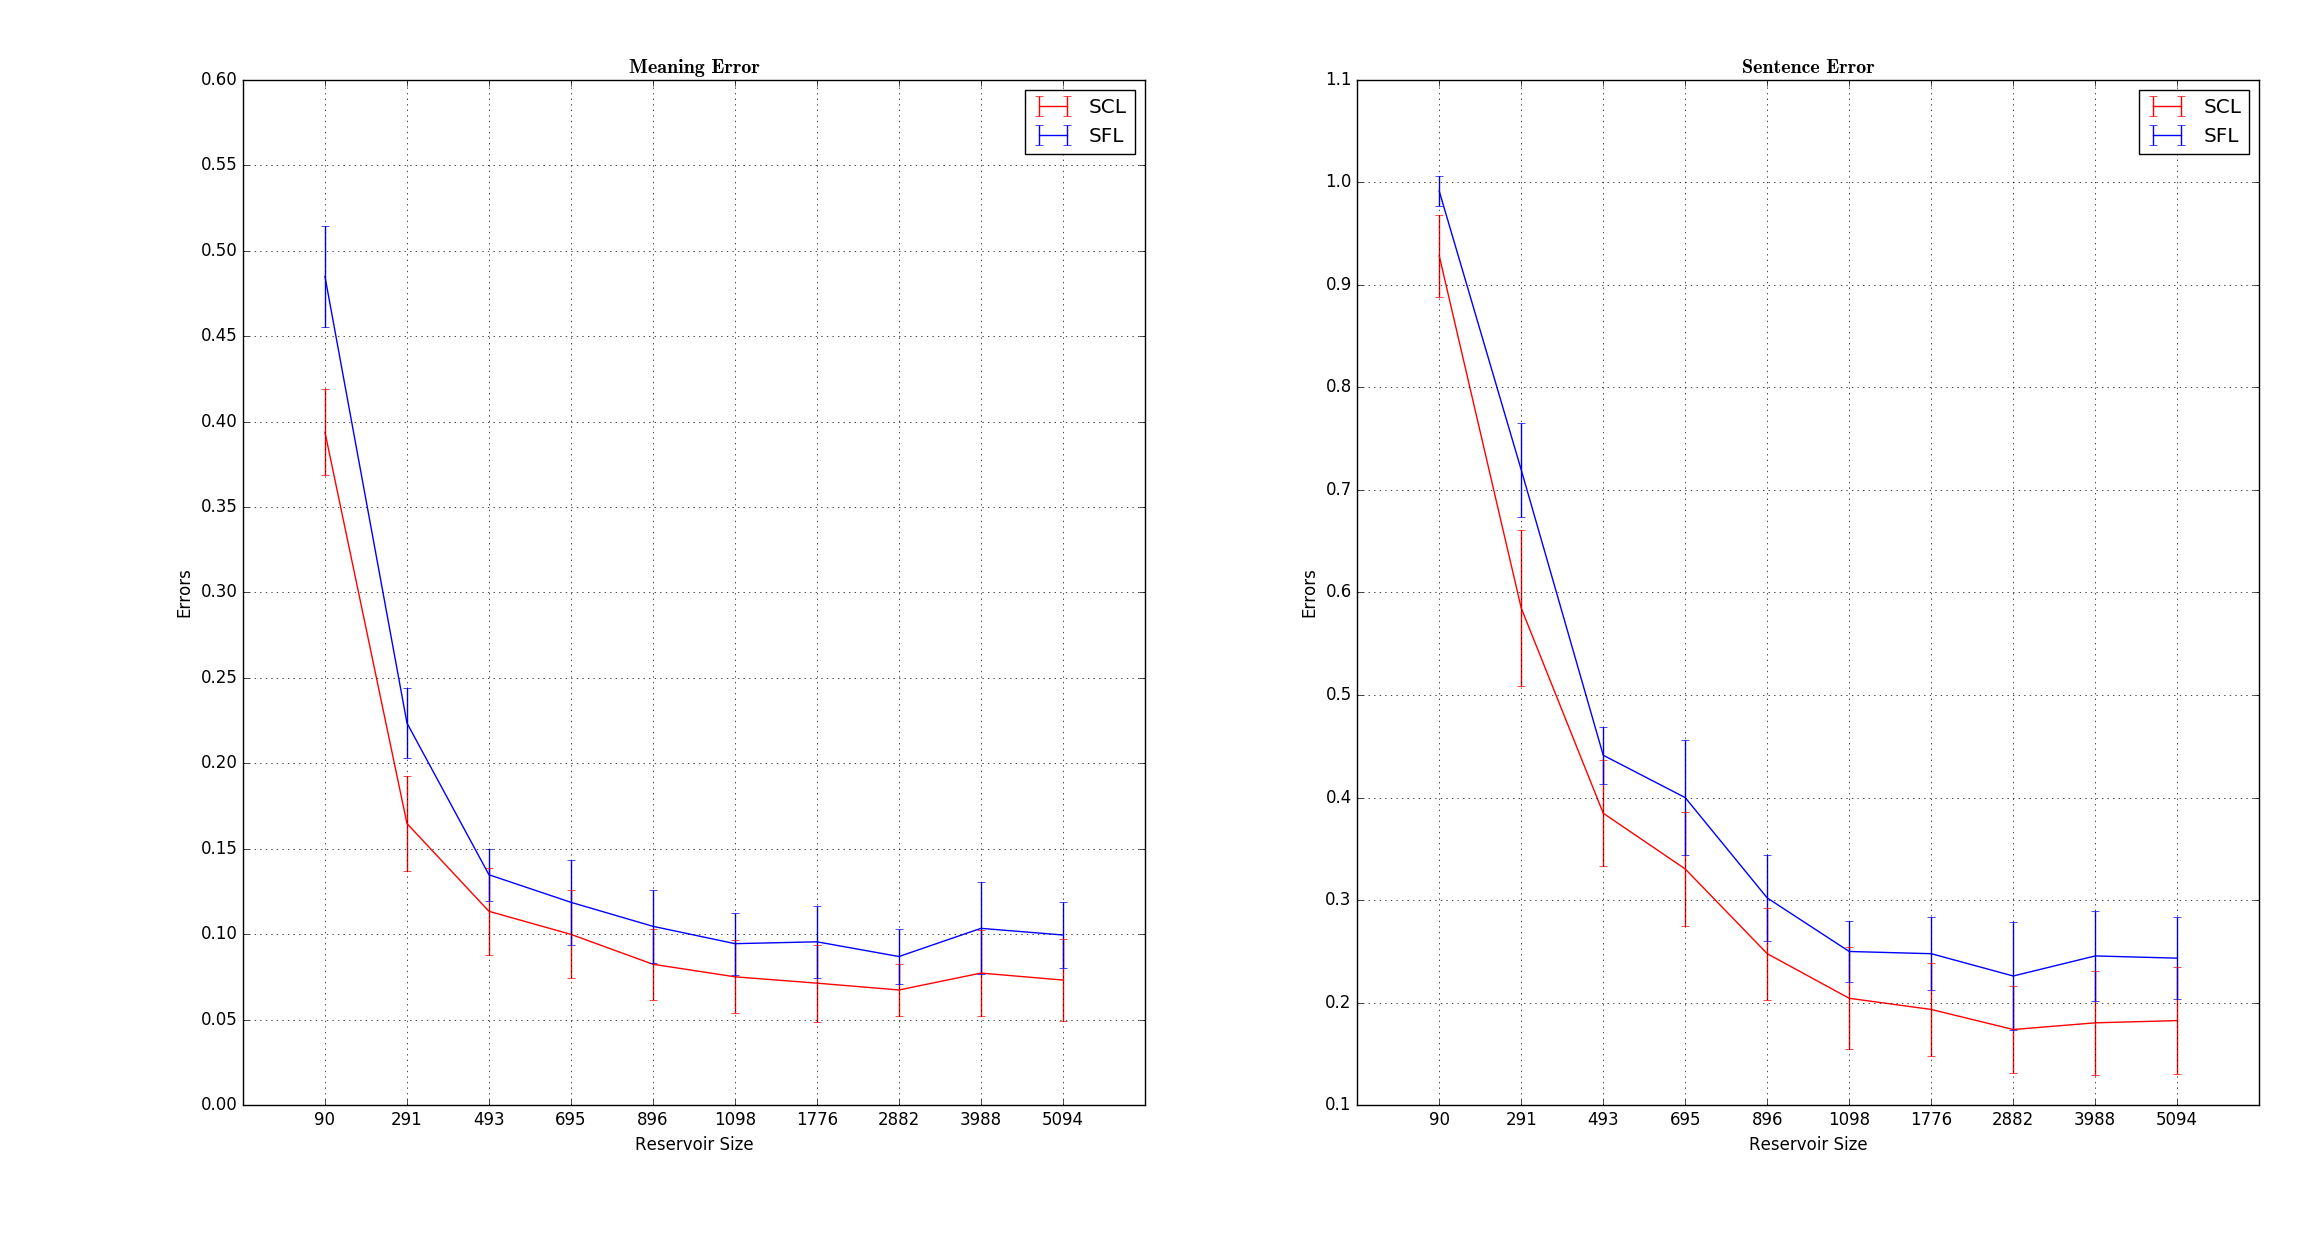
\includegraphics[width=1.0\linewidth]{reservoir_size_1}
\caption{\textbf{Effect of reservoir size on cross validation errors on Model Variant-1:} Description goes here.}
\label{fig:reservoir_size_1}
\end{figure}

We also studied the effect of reservoir size on the performance of model variant-2 when using word2vec word embeddings and also when using grammatical construction of sentence along with localist word representation. In figure \ref{fig:reservoir_size_2}, it can be clearly observed that the model variant-2 performs much better with word2vec word embeddings with all reservoir size when compared to use grammatical construction of sentence with localist word vector. Even the highest F1-Score ($F1 = 80.06 \%$) obtained using localist representation with reservoir size 2250 is much less than that of obtained using word2vec word embeddings with reservoir of size 200 (F1 = $ 93.56\%$). Overall with increase in reservoir size the classification score also increases irrespective of the word vectors used as an input to the model. The model also asymptotes when reservoir size is 200 and 600 with word2vec and localist vectors respectively, indicating that model can not be genralized further on this corpus (i.e. corpus-462). 

\begin{figure}[hbtp]
\centering
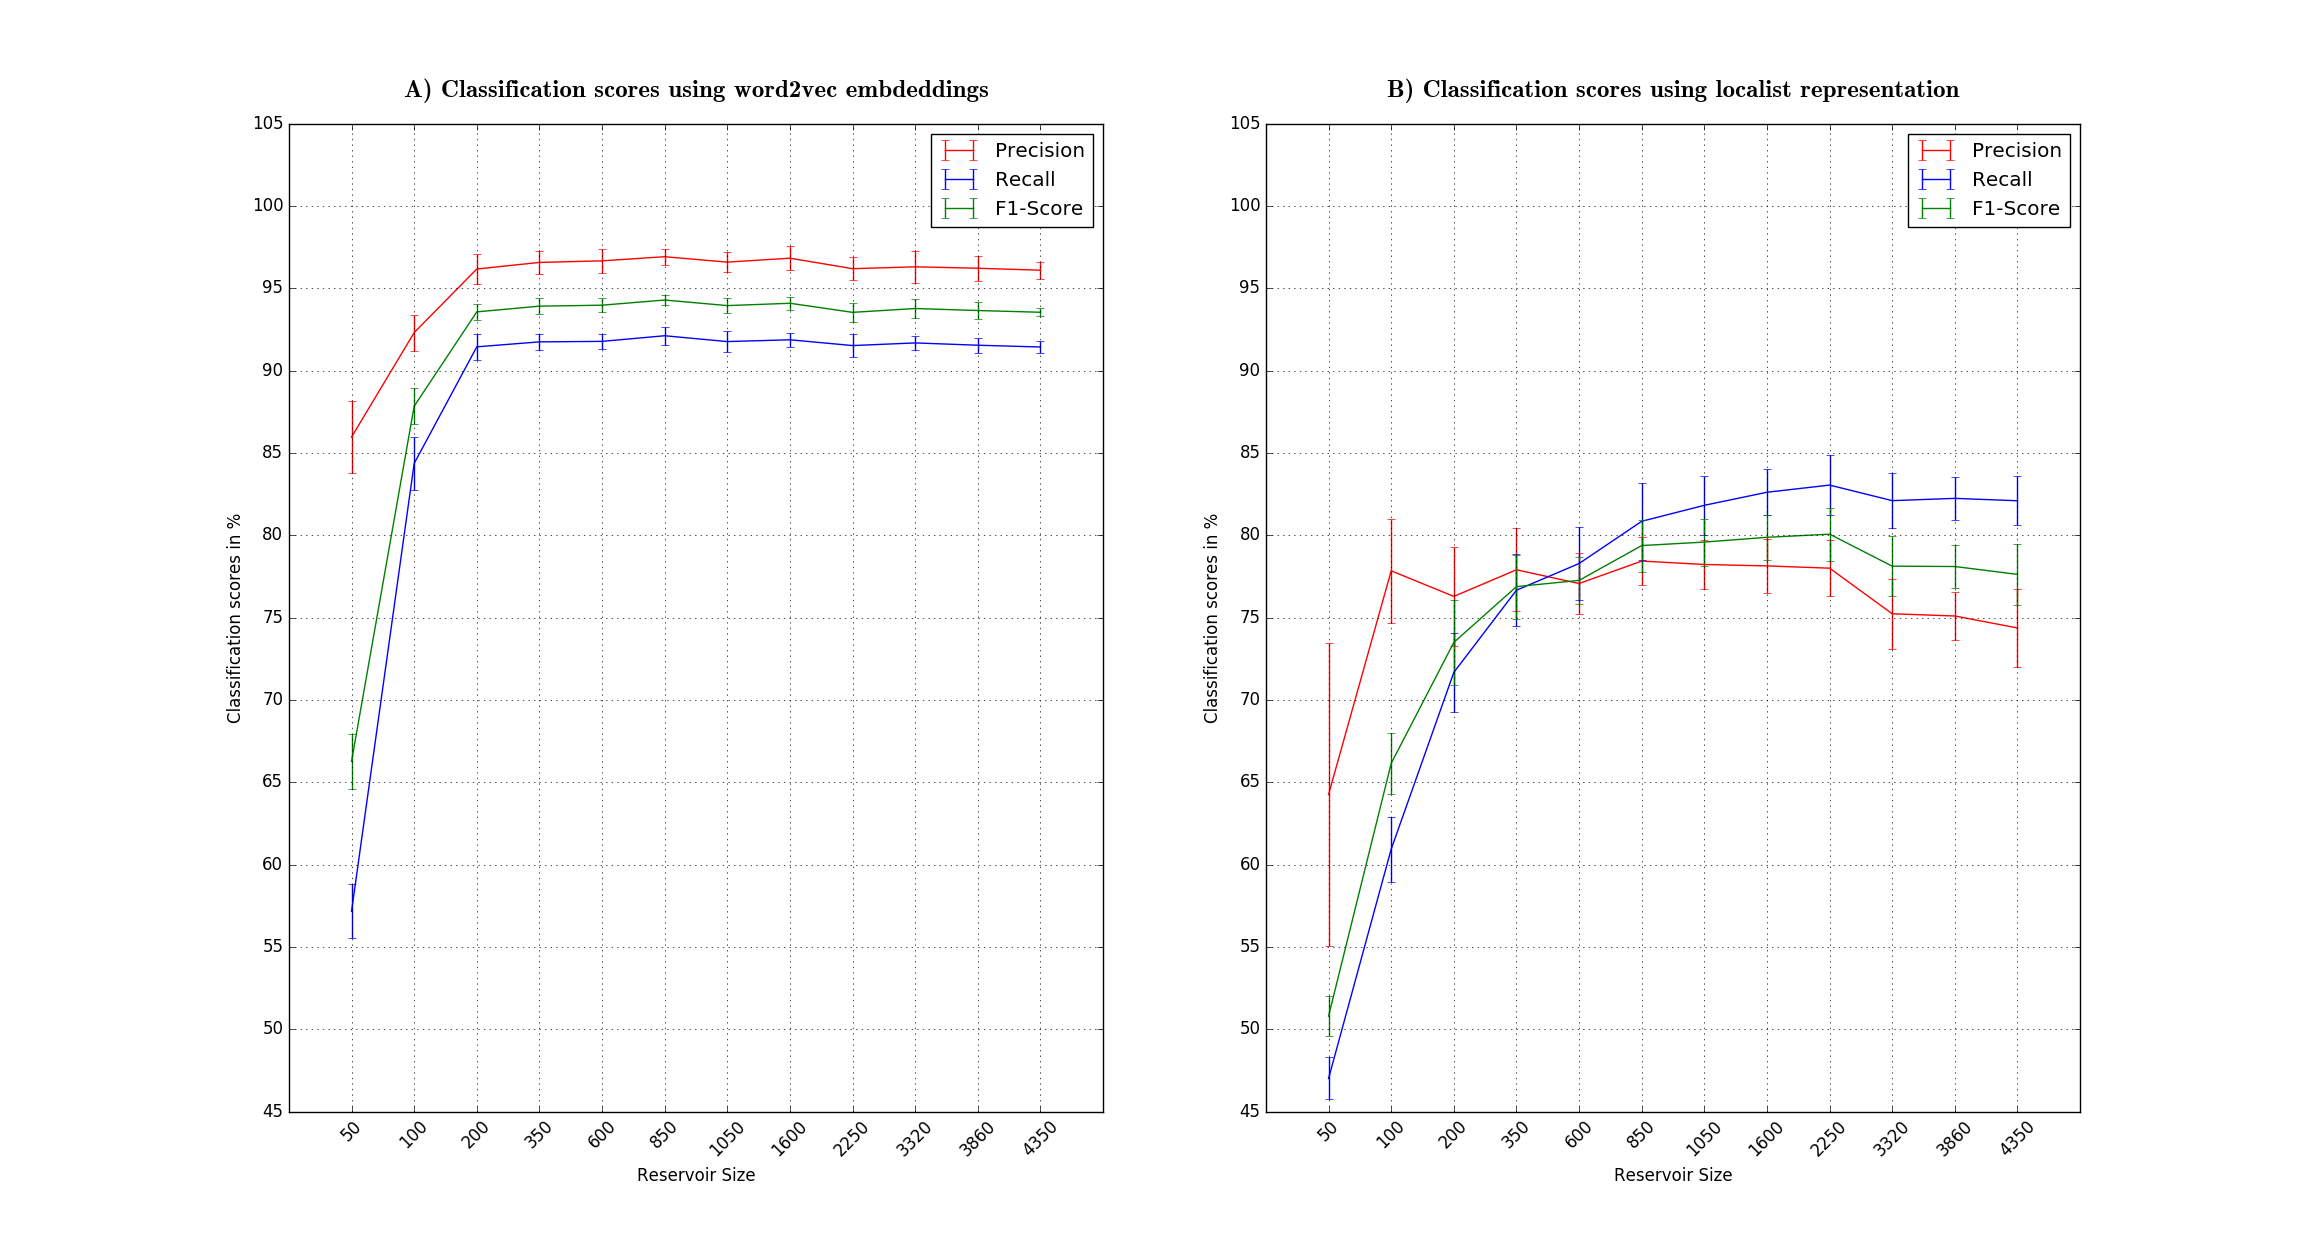
\includegraphics[width=1.0\linewidth]{reservoir_size_2}
\caption{\textbf{Effect of reservoir size on classification scores of Model Varinat-2:} Description goes here.}
\label{fig:reservoir_size_2}
\end{figure}



%TODO: Write the effect of reservoir size on the model variant-2

\subsection{Experiment-5: Effect of Corpus size}

In the previous experiments we noticed that the errors rates with Word2Vec-ESN model and classification scores model variant [] improved as we extended the corpus size from 45 to 462 sentences. To investigate the effect of corpus size and scaling capability of the model, we used extended corpus-90582(see section) for this experiment. As the corpus also contains $12\%$ of ambiguous sentences which impede the learning and generalization of the model, this experiment will also validate the model's ability to process the abmbiguous sentences.

In order to study the generalization capabilty of the model with different corpus size,  6 sub-corpora were created by randomly sampling $6\%$, $12\%$, $25\%$, $50\%$, $75\%$, $100\%$ of sentences from the orginal corpora of 90582 sentences\cite{end-to-end}. Each of the sub-corpora was exposed to the model and 2-fold cross validation is performed where the model was trained on half the sub-corpora size and tested on remaining half. The second half used for testing was then used to train the model and then tested on the first half used for training previously.

Figure \ref{fig:corpus_size_1} shows the cross validation errors rates with respect to corpus size while using model variant-1. It can be observed that with increase in corpus size from $6 \%$  to $25 \%$, the meaning error sharply drops from some $12.23 \%$ to $3.92 \%$ in SCL mode and from $12.10\%$ to $4.88 \%$ in SFL mode. Similarly, the sentence error also decreases from $54.43 \%$ to $21.89 \%$ in SCL and from $55.22 \%$ to $26.17 \%$ in SFL mode. When the sub-corpora size is $50\%$, where the model was trained only on $25\%$ of corpora size, the model already generalized with $17.11 \%$ sentence error and $2.98 \%$ meaning error in SCL mode and  $22.32 \%$ sentence error and $4.13 \%$ meaning error in SFL mode. The more gradual slope from $50 \%$ to $100 \%$ sub-corpora size in both the learning modes for meaning and sentence error indicates the model has already generalized and further increase in corpus size won’t have much effect on cross validation error.
 

\begin{figure}[hbtp]
\centering
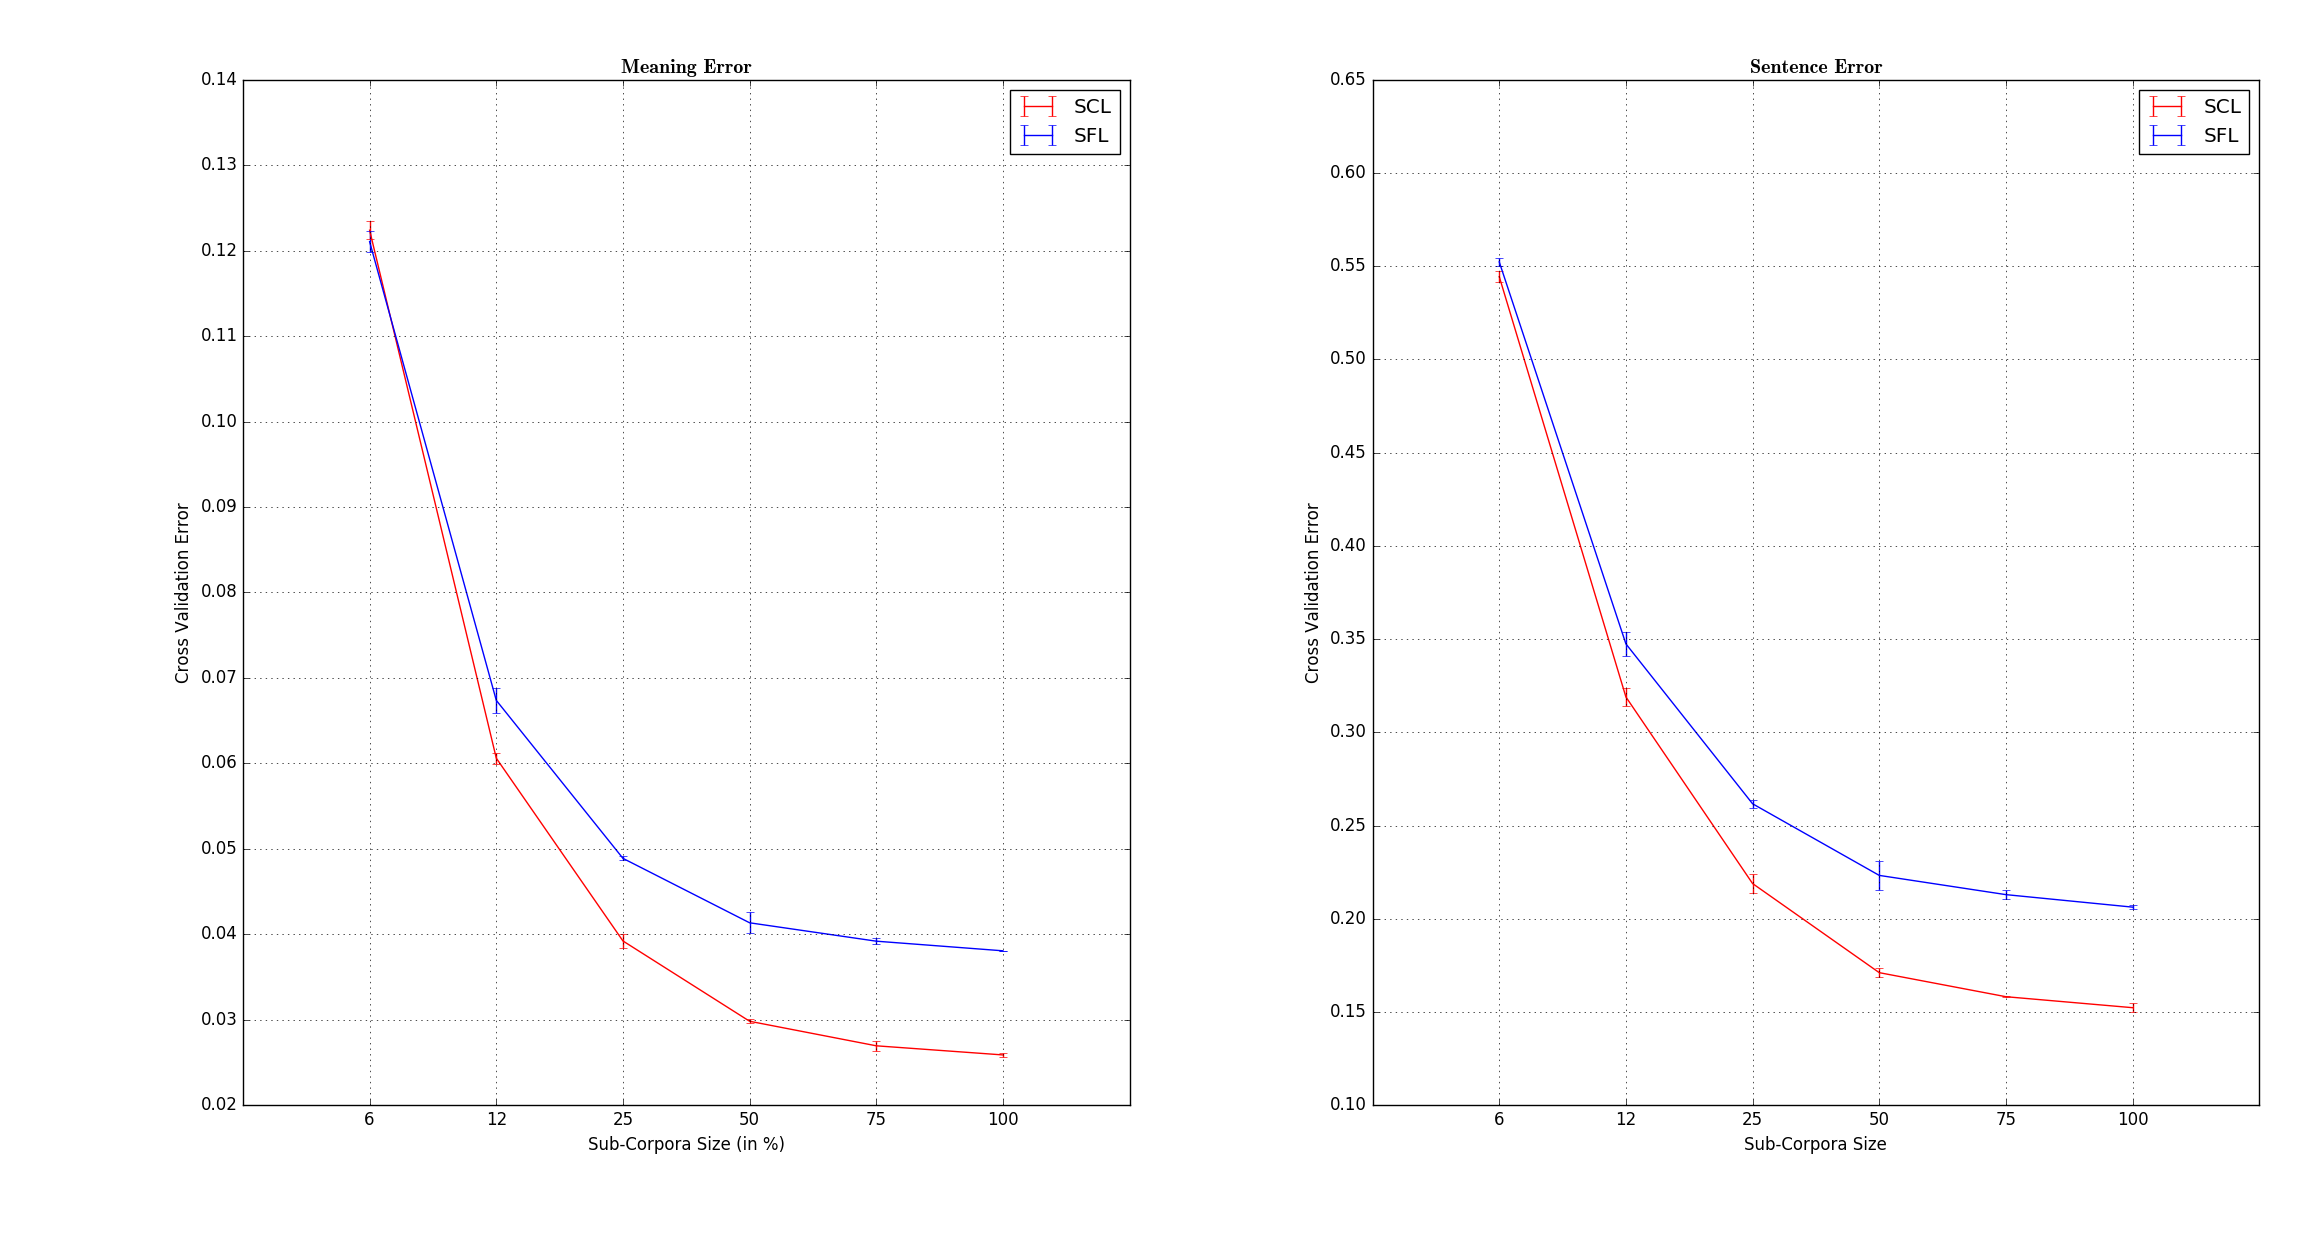
\includegraphics[width=1.0\linewidth]{corpus_size_1}
\caption{\textbf{Effect of corpus size on cross validation errors:} Description goes here.}
\label{fig:corpus_size_1}
\end{figure}


\begin{figure}[hbtp]
\centering
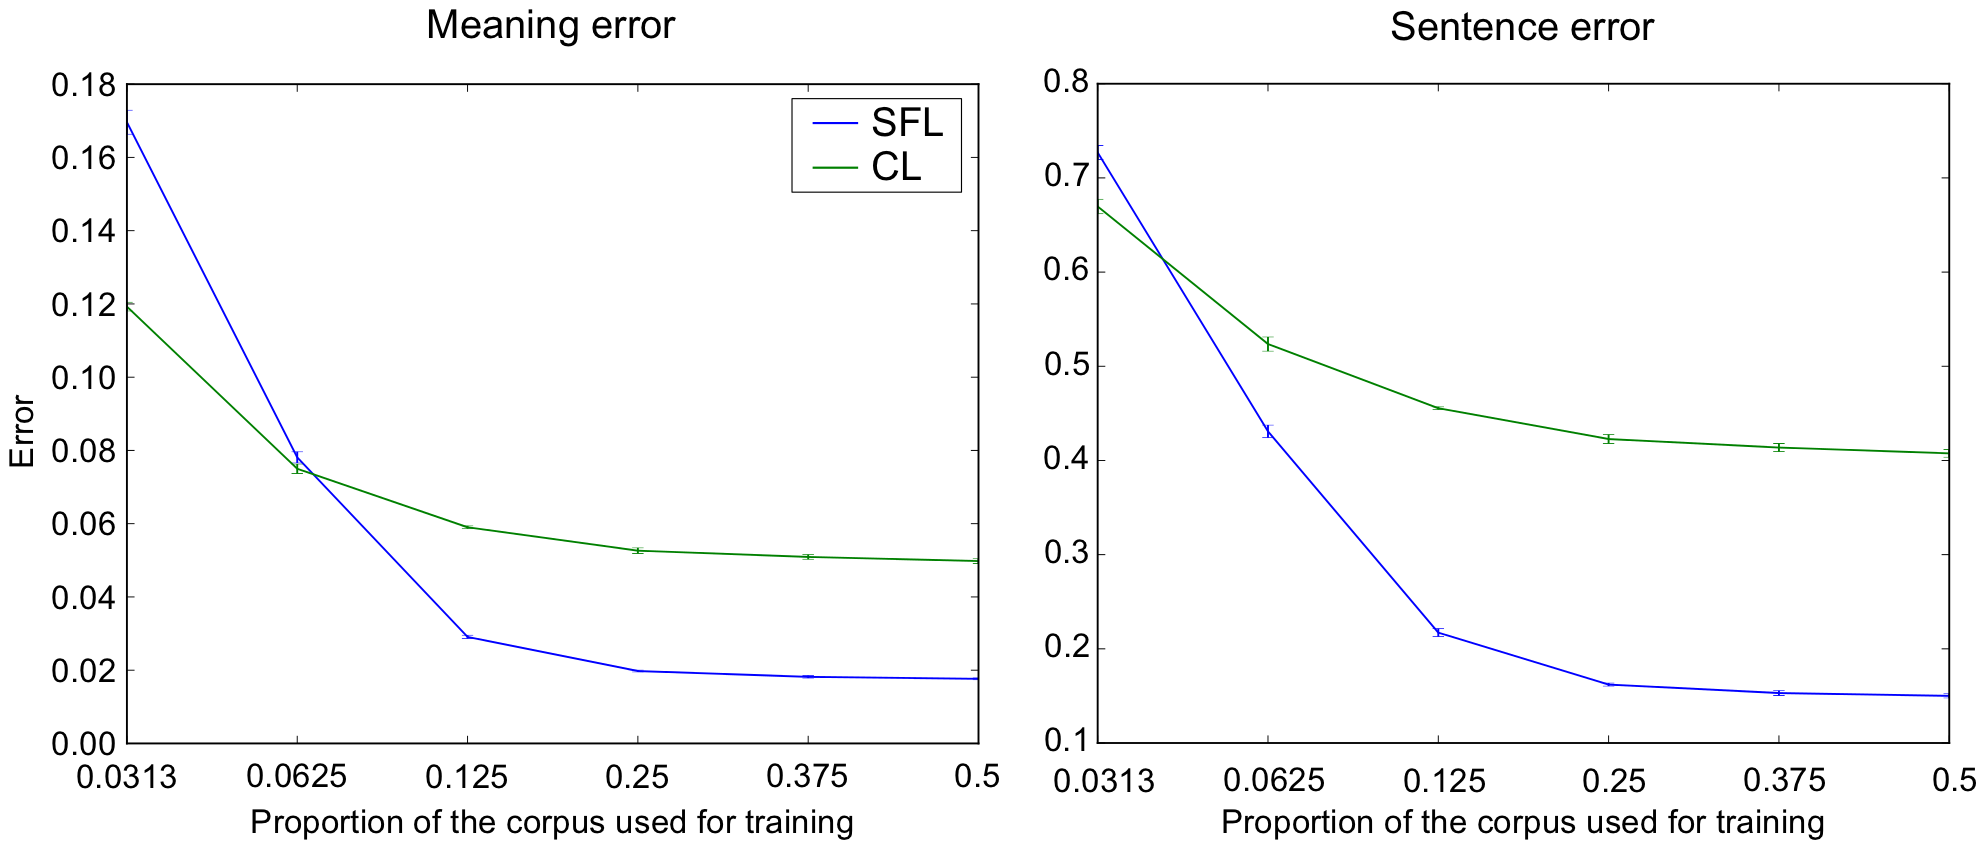
\includegraphics[width=1.0\linewidth]{corpus_size_xavier}
\caption{\textbf{Effect of corpus size on cross validation errors using localist word vector as reported in [ref?]:} Description goes here.}
\label{fig:corpus_size_xavier}
\end{figure}


\newpage

\subsection{Experiment-6: Neural output activity of the model}

In the previous experiments we observed that both the model variants generalized well and cross validation error rates dropped with increase in reservoir size. As we saw that model variants performs better when we increased corpus size from 45 sentences to 462 sentences. As corpus-45 contains sentence with uniques grammatical structure (i.e. active, passive, subject and object relative etc.) we added these 45 sentences to corpus-462 so the resultant corpus have 507 sentence (462+45) and analysed the activation produced by model variant-1 for the input sentences. We observed that while learning the model is re-analyzing the thematic roles across the time. The same behaviour was observed by xavier et. al [ref?] with sentences in grammatical constructions form and localist representation of words. However we observed that the model is making earlier predictions with word2vec embeddings. The reason for such a behavior is because the word2vec word embeddings were learned from the context words and each word vector encodes the information about neighbouring words. 

We examined and plotted the four sentences with active and passive constructions studied in Hinaur et al. [ref].

\begin{enumerate}[noitemsep]
\item the man gave the book to the boy. \label{eg-1:or-sent-17}
\item the man took the ball that hit the glass. \label{eg-1:or-sent-23}
\item the boy caught the ball that was thrown by the man.  \label{eg-1:or-sent-27} 
\item the ball was pushed by the man.  \label{eg-1:or-sent-16}
\end{enumerate}

Figure \ref{fig:act_analysis_1} shows the activations for these four different sentences across time. As all the four sentences start with "the", activation at this word is same for all the sentences. In sentences \ref{eg-1:or-sent-17} and \ref{eg-1:or-sent-23} with the arrival of first noun (i.e. man) the activation of noun-2 (i.e. book and ball) being an object of verb-1 is increased and confirmed with arrival of verb 'gave' and 'took' respectively.

\begin{figure}[hbtp]
\centering
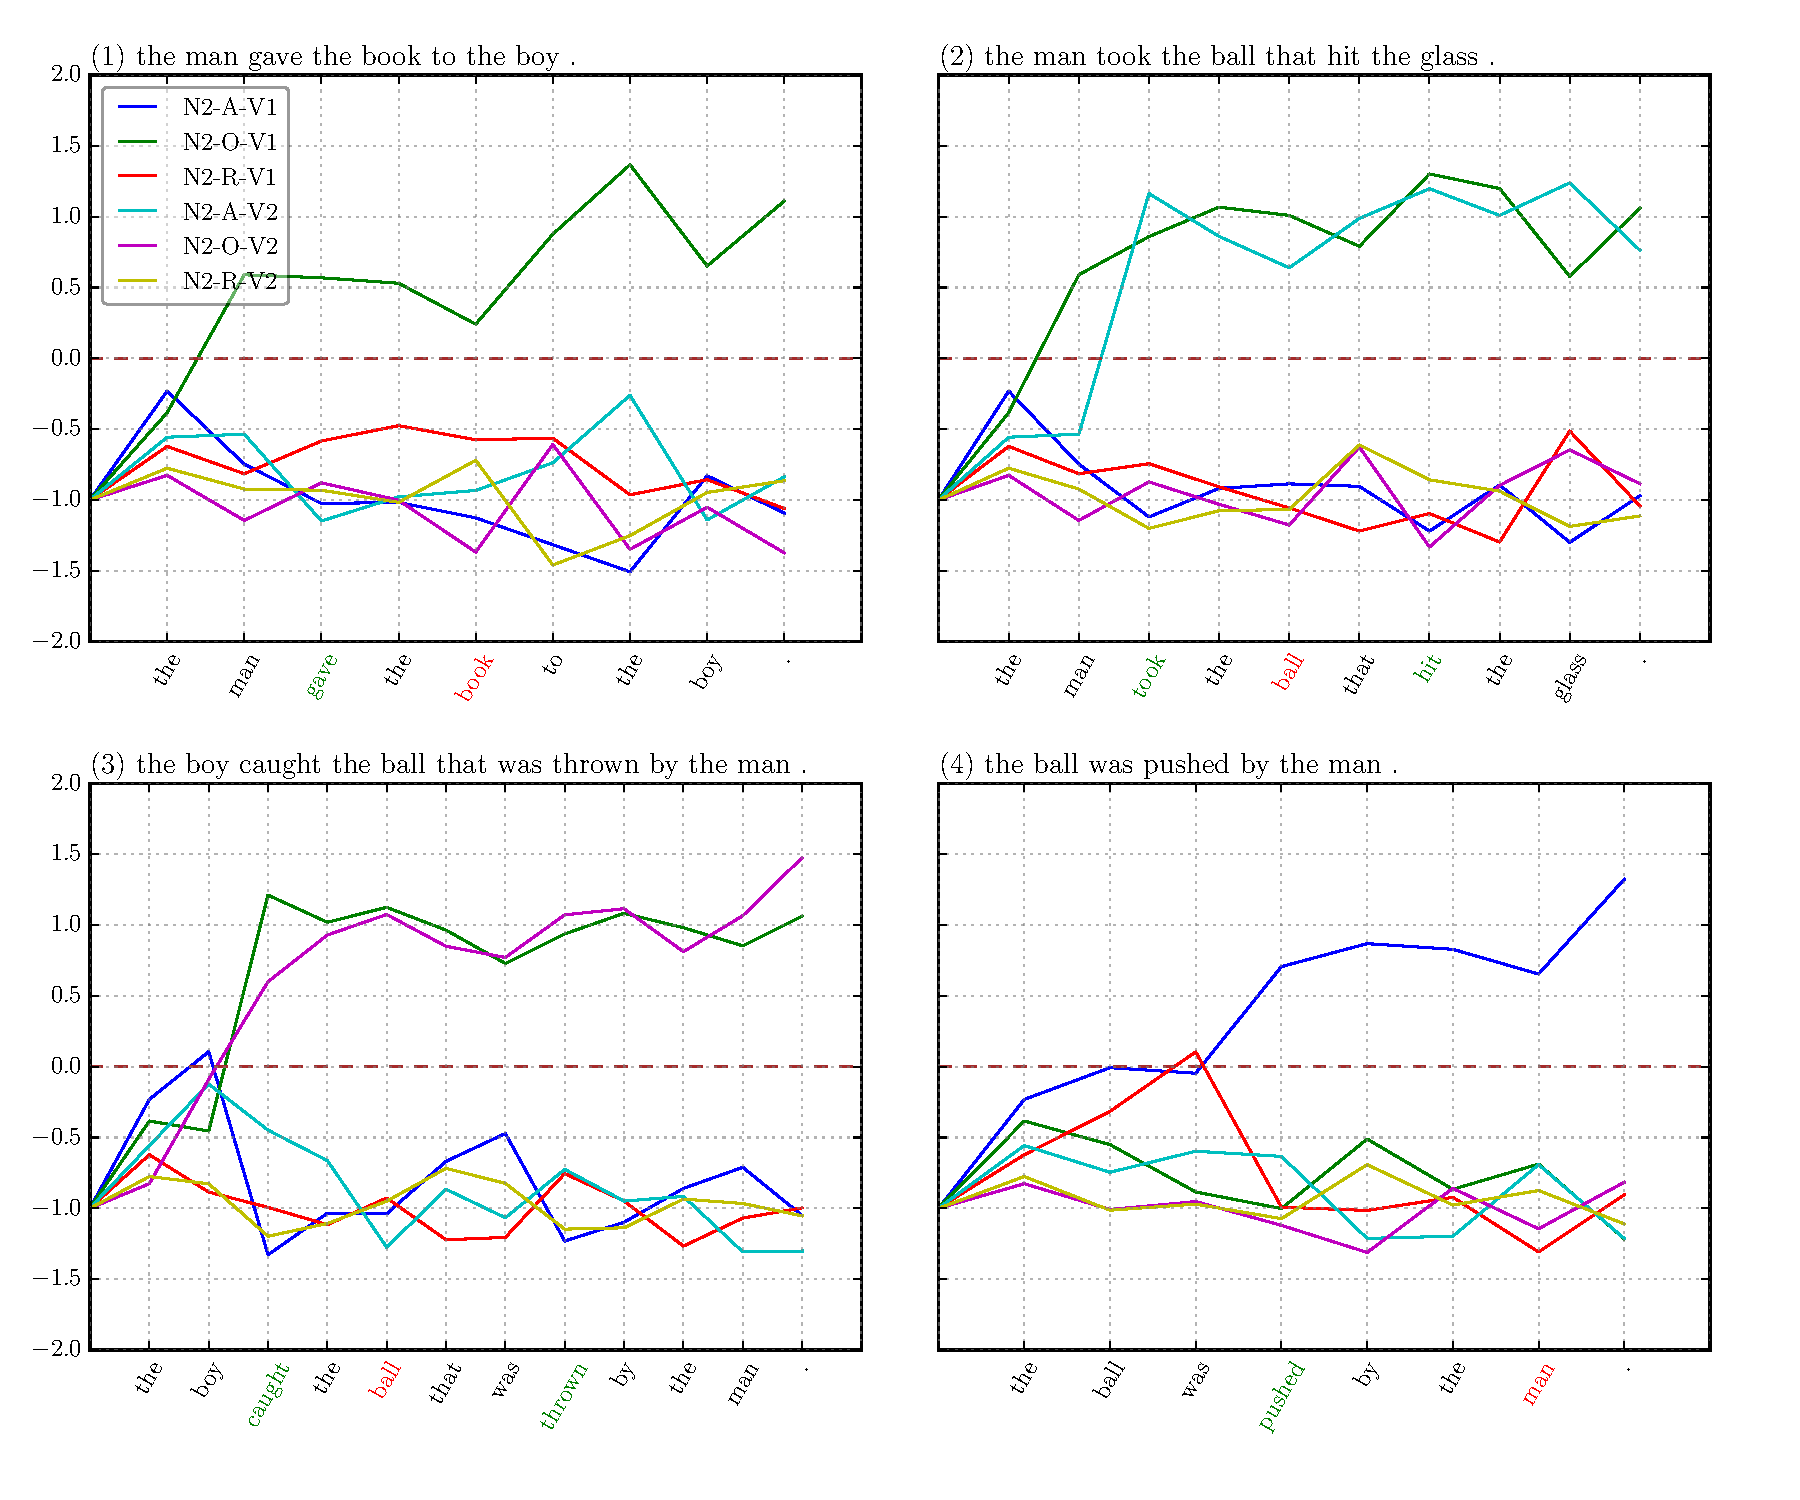
\includegraphics[width=1.0\linewidth]{act_analysis_1}
\caption{\textbf{Effect of corpus size on cross validation errors using localist word vector as reported in [ref?]:} Description goes here.}
\label{fig:act_analysis_1}
\end{figure}

Consider another two sentences 
\begin{enumerate}[noitemsep]
\item the dog that chased the cat ate the rat \label{eg-1:or-sent-17}
\item the cat that the dog chased bit the man. \label{eg-1:or-sent-23}
\end{enumerate}


\begin{figure}[hbtp]
\centering
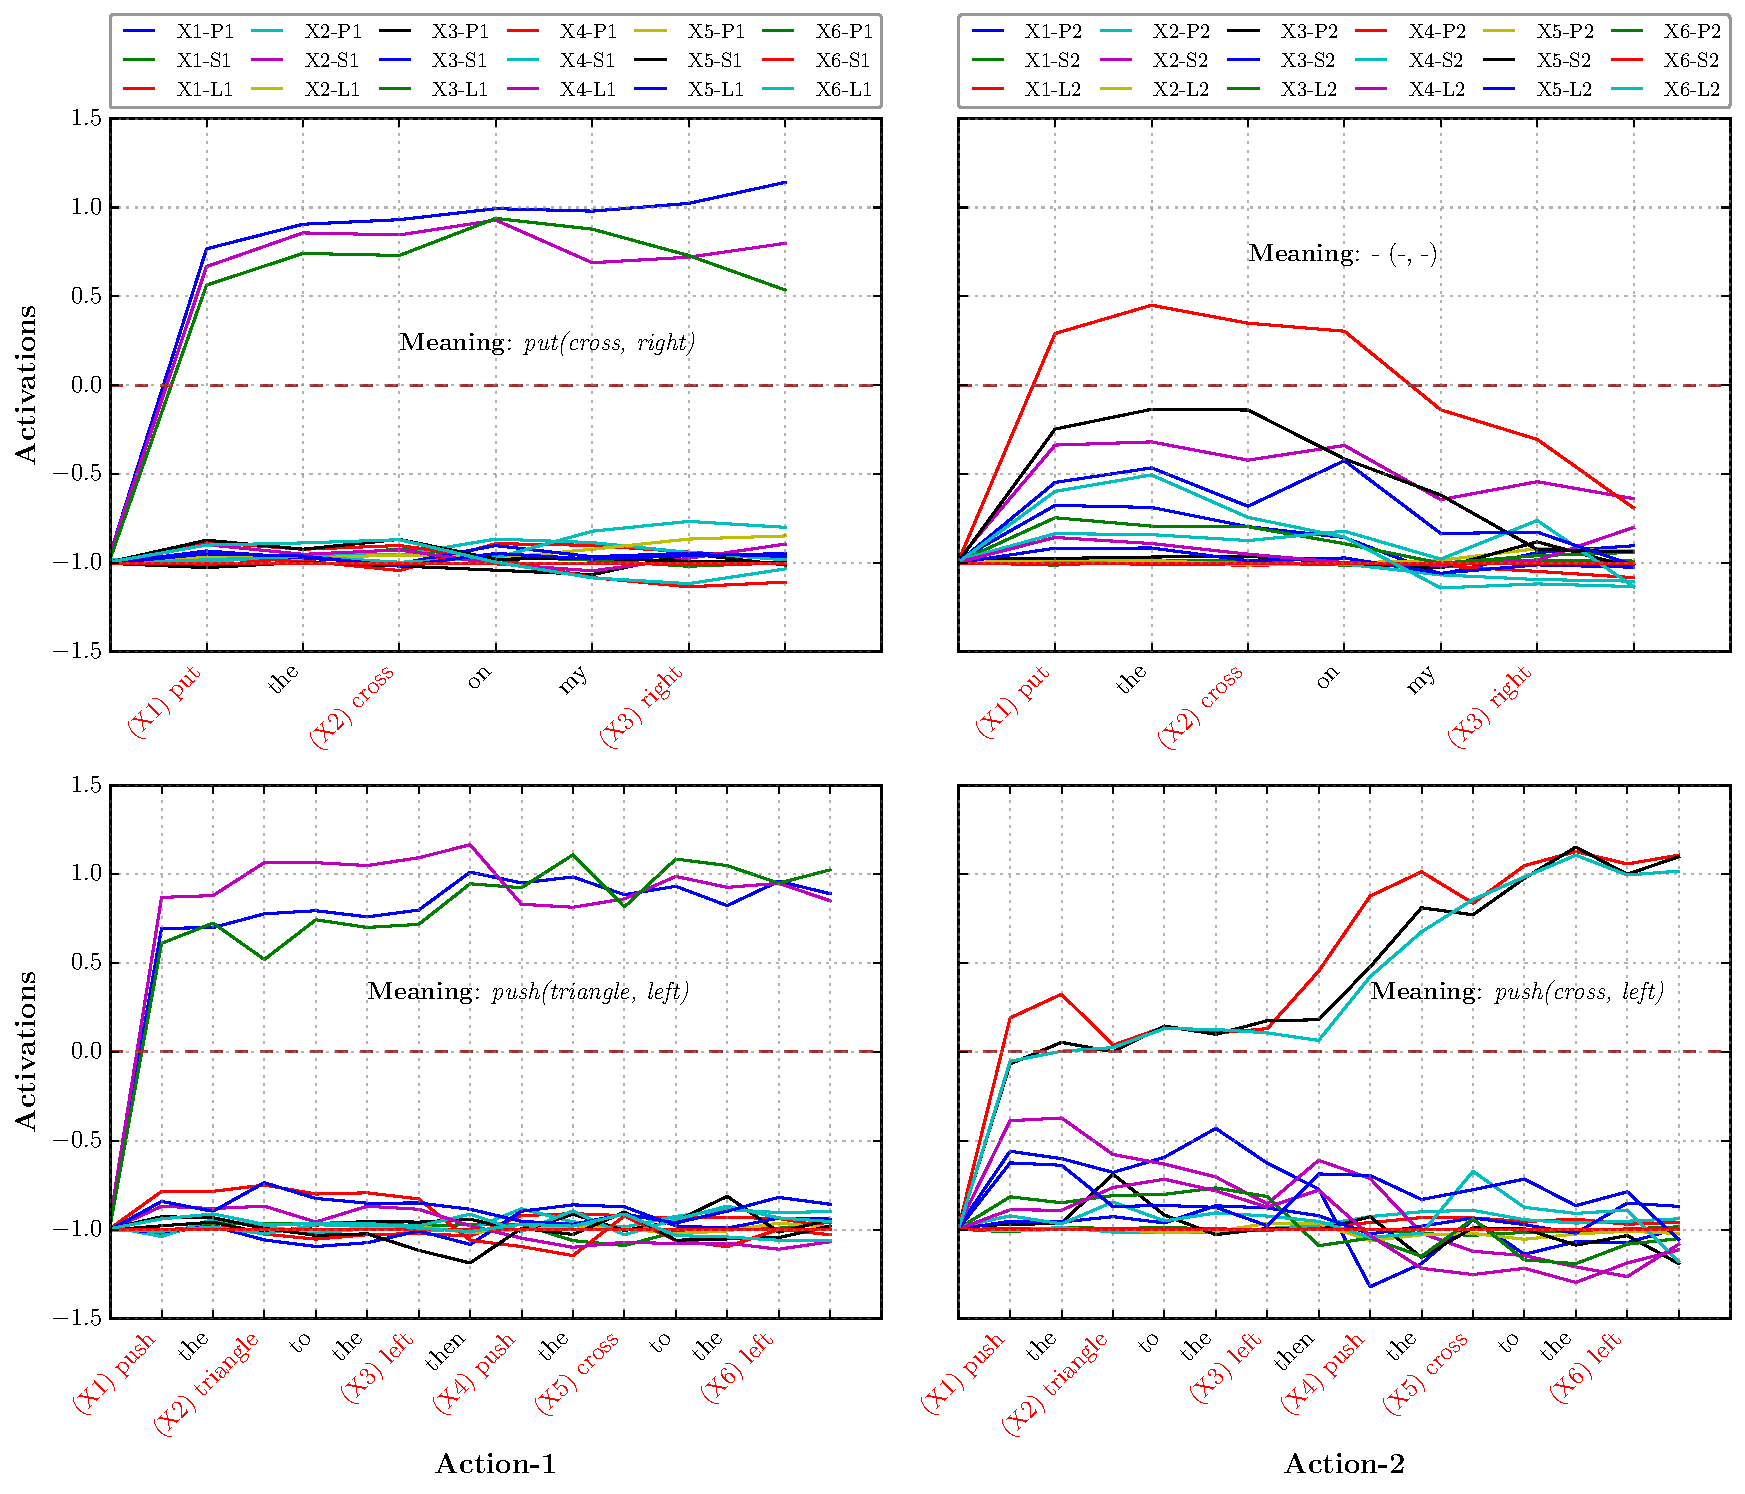
\includegraphics[width=1.0\linewidth]{act_analysis_2}
\caption{\textbf{Effect of corpus size on cross validation errors using localist word vector as reported in [ref?]:} Description goes here.}
\label{fig:act_analysis_2}
\end{figure}

\begin{figure}[hbtp]
\centering
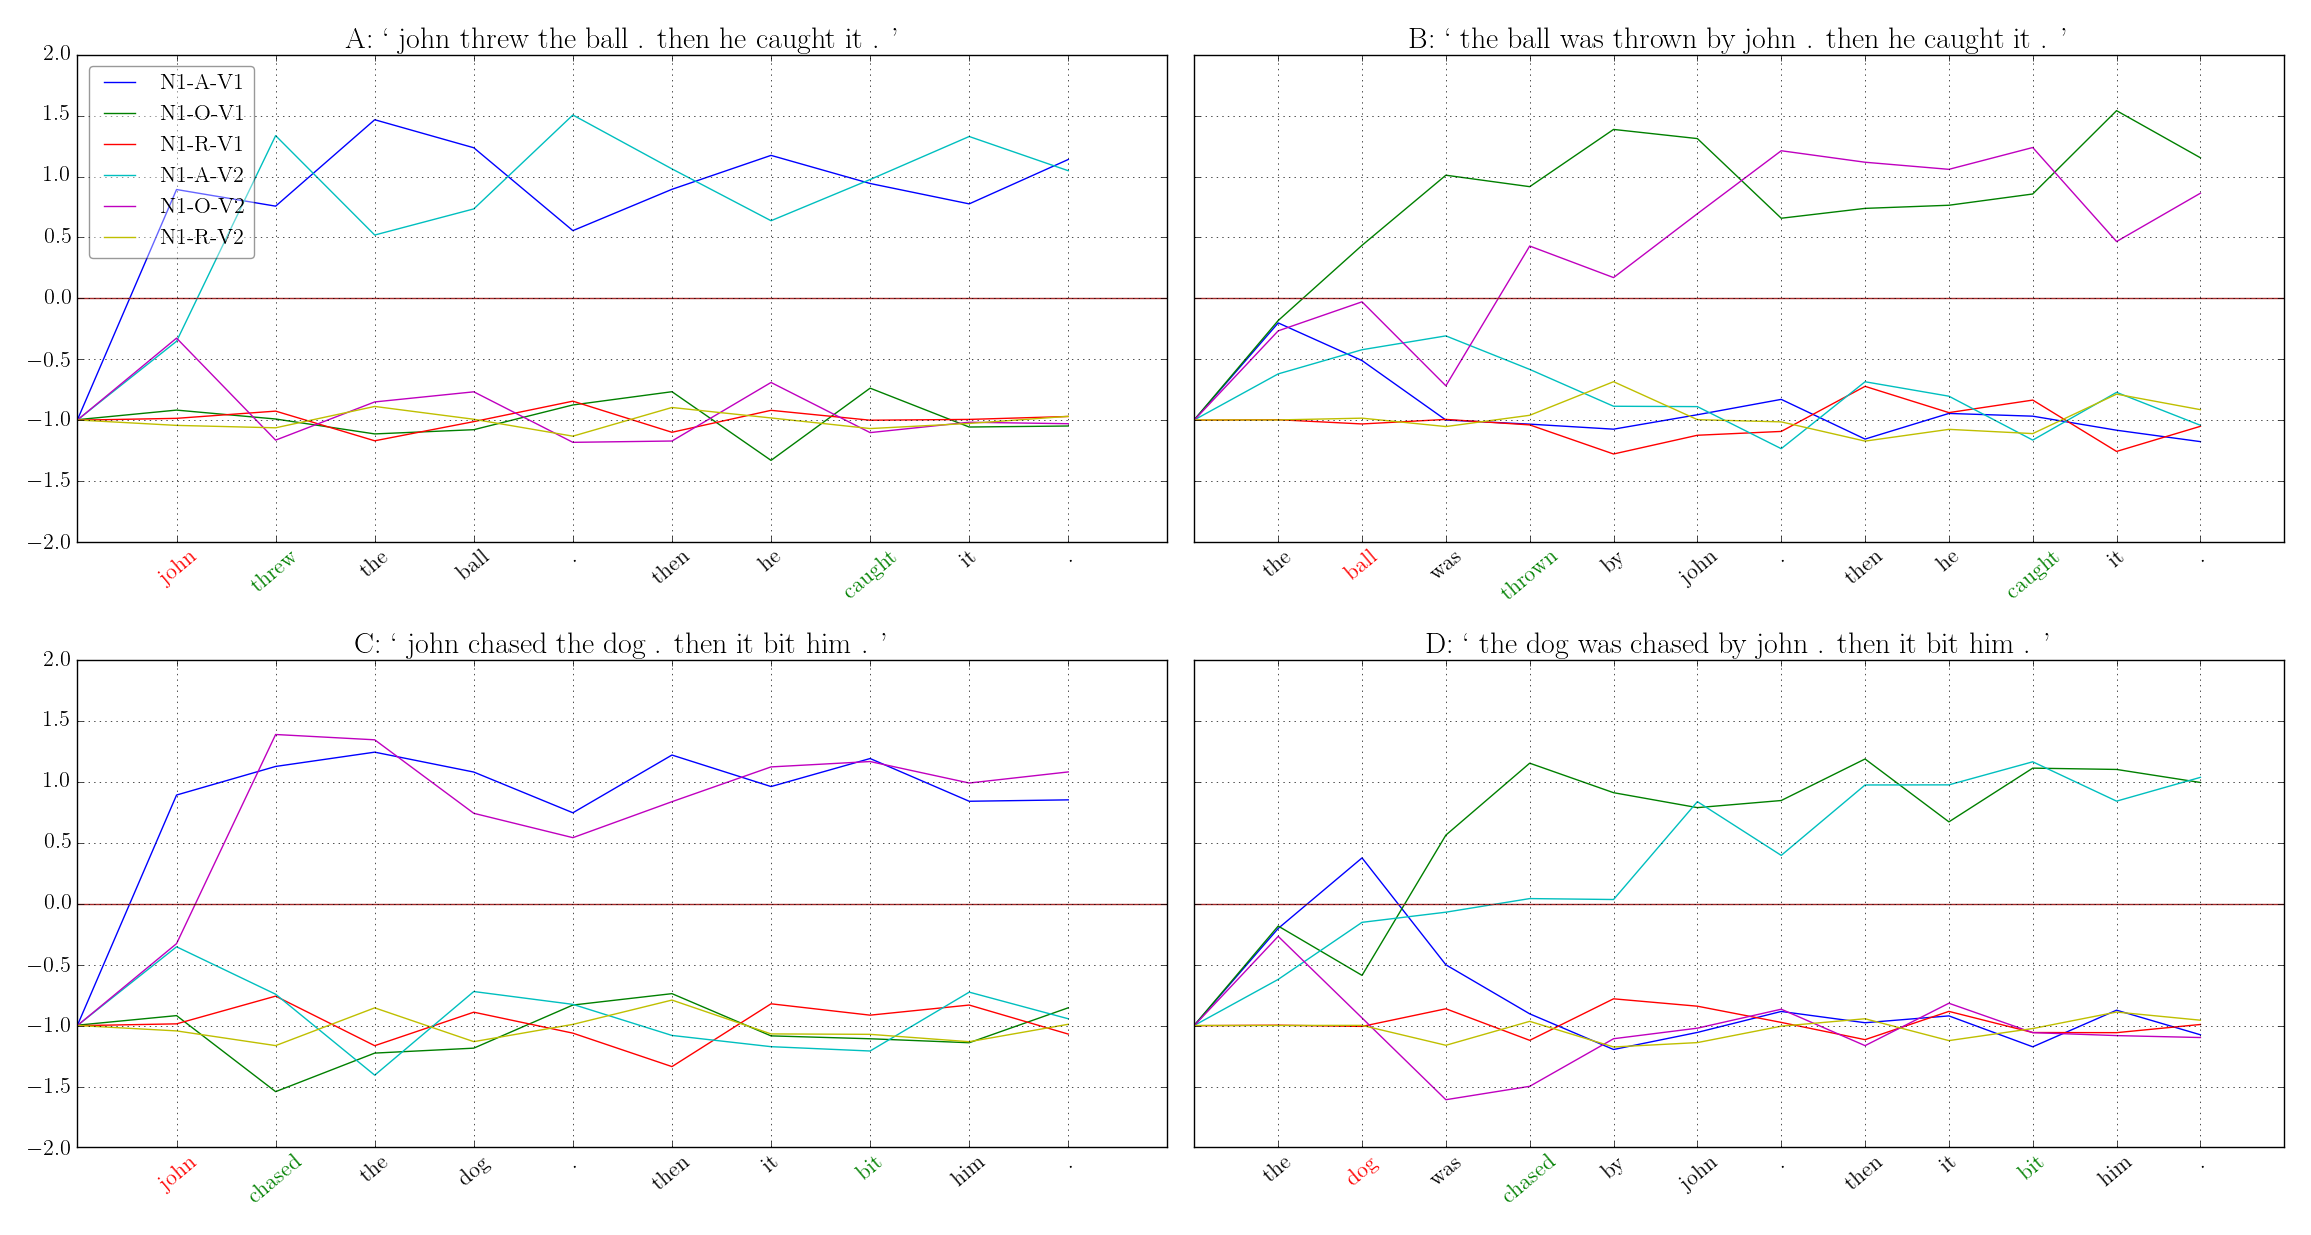
\includegraphics[width=1.0\linewidth]{act_analysis_3}
\caption{\textbf{Effect of corpus size on cross validation errors using localist word vector as reported in [ref?]:} Description goes here.}
\label{fig:act_analysis_3}
\end{figure}


\subsection{Experiment-7: Generalization on new corpus}

One may argue that the previously used corpus (corpus-462 and corpus-90k), which were artifically constructed using grammer is adding a bias to the model which makes it easier for the model to learn and genralize on these corpus. To answer this question, in this experiment we used the corpus collected by Hinaut et al. \cite{tra:tra:xavier_hri} in a Human Robot Interaction (HRI) study of language acquisition. The sentences in the corpus were collected from the real subjects interacting with the humanoid robot (iCub). The corpus contains 373 complex instruction to perform single or double actions with temporal correlation (see action performing task in Experiments of \cite{tra:tra:xavier_hri} for more details). For example, "Point to the guitar" is a one action command whereas "Before you put the guitar on the left put the trumpet on the right" is a complex instruction with double action, where second action is specified before the first action. Thus this data is complex enough to test the learnabilty and generalization of the model.  

To test the generalization of Word2Vec-ESN model on this corpus, leave-one-out (LoO) cross validation was performed. We chose LoO, so that results can be compared with that of obtained in $\theta RARes$ model of	Xavier et al.  \cite{tra:tra:xavier_hri}. As illustrated in table \ref{tab:corpus_373}, it can be observed that while using word2vec word embeddings over grammatical form and localist word vectors, of the input sentence, error improved by $26.31 \%$, $17.97 \%$ sentence error with 500 and 1000 reservoir neurons respectively. It can also be observed that with increase in reservoir size the sentence error also decreases. For this experiment we did not explore for the best parameters, but instead we used the optimized parameter obtained on corpus-462 in experiment 2 i.e. SR = 2.4, IS = 2.5 and LR = 0.07. This shows that previously learned model parameters are capably roboust enough to generalize on new corpus. 

\begin{table}
\centering
\begin{threeparttable}
\caption{Generalization error in sentence continuous learning mode for corpus-373.}
\label{tab:corpus_373}
\rowcolors{2}{gray!25}{white}
\begin{tabular}{llll}
\toprule
Reservoir 	 		& Sentence Error 	&  Word2Vec-ESN 		& $\theta RARes$ \\
\midrule                 
\textbf{500 N}		& mean(std.) 		& 42.65 ($\pm$ 1.36) 	& 68.96 ($\pm$ 2.03)  \\
					& Best 				& 26.54 				& 44.50  \\
\textbf{1000 N}		& mean(std.) 		& 40.29 ($\pm$ 1.13) 	& 58.26 ($\pm$ 1.37)\\
					& Best 				& 25.73 				& 34.85 \\
\bottomrule
\end{tabular}
\begin{tablenotes}
\small
\item 
Sentence errors (in $\%$) obtained with Word2Vec-ESN model and $\theta RARes$ in SCL mode for input sentences with reservoir of size 500 and 1000 neurons. The results reported are mean and standard deviation of 10 reservoir instances. The best error here means the count of sentence errors common in all 10 reservoir instances\cite{tra:xavier_hri}.  
\end{tablenotes}
\end{threeparttable}
\end{table}